\documentclass{article}
\usepackage{graphicx}
\usepackage{geometry}
\usepackage[MeX]{polski}
\usepackage[polish]{babel}
% Make header with name and date etc.
\usepackage{fancyhdr}
\lhead{Zuzanna Cienka\\nr albumu 148201}
\rhead{\today\\Programowanie obiektowe}
\thispagestyle{fancy}
\renewcommand{\abstractname}{}    % clear the title
\usepackage[utf8]{inputenc}
\setlength{\parindent}{0pt} % Don't indent new paragraphs
\setlength{\headheight}{24pt} 

\begin{document}

\begin{center}\vspace{-1cm}
    \textbf{ \huge Go}\\~\\
    \large Projekt zaliczeniowy Java\\
\end{center}

% \noindent
Celem gry jest otoczenie największego terytorium planszy. Gracze
naprzemniennie układają na przecięciach planszy 19x19 białe i czarne kamienie.
Grę rozpoczyna gracz, który wybrał czarne kamienie, a miejscie kamieni nie
może zostać zmnienione, chyba, że zostaną przechwycone przez przeciwnika.
Przechwycenie polega na otoczeniu kamieni przeciwnika. Gra kończy się gdy
gracze pominą ruch po sobie lub jeden z graczy zrezygnuje. Punkty są
obliczane jako różnica obszarów planszy otoczonych przez kamienie danego
gracza i przechwyconych kamieni.\\

\begin{enumerate}
    \item Plansza goban
    Plansza goban składa się z 19 poziomych i 19 pionowych linii i jest 
    otoczona współrzędnymi składającymi się z liter od A do T 
    (brak litery I, ponieważ przypomina ona cyfrę 1 w zależności od
    czcionki) oraz cyfr od 1 do 19. Pomiędzy przecięciami linii 

    \begin{center}
        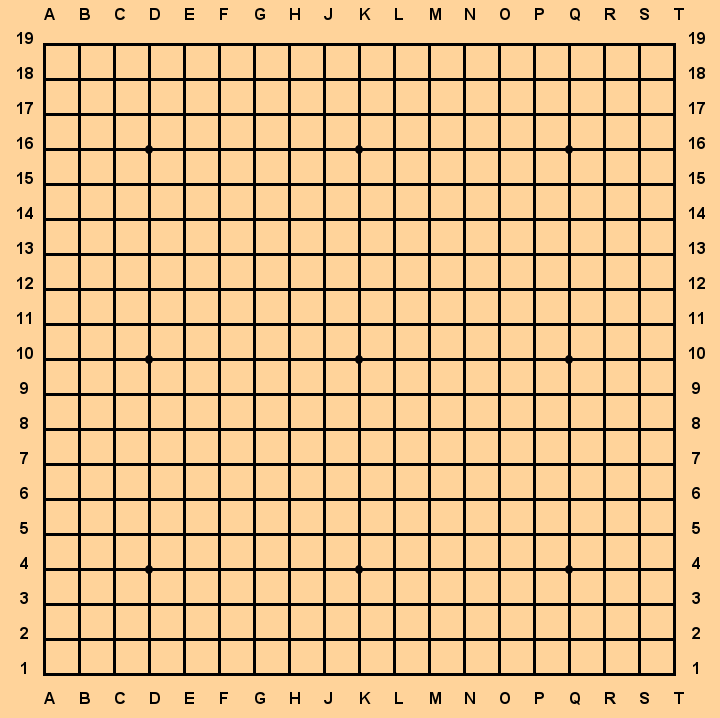
\includegraphics{imgs/goban.png}
    \end{center}
    \item Przechwytywanie kamieni\\
    Mechanizm przechwytywania kamieni został zrealizowany z wykorzystaniem
    algorytmu flood fill.\\
    Przykłady:\\
    \begin{center}
        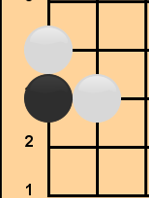
\includegraphics{imgs/capture1a.png}
        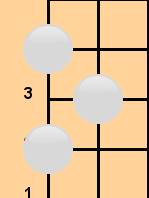
\includegraphics{imgs/capture1b.png}
    \end{center}
    \begin{center}
        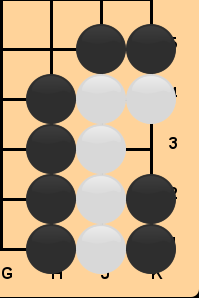
\includegraphics{imgs/capture2a.png}
        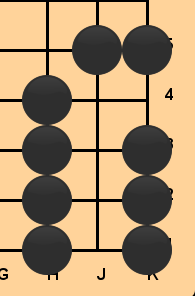
\includegraphics{imgs/capture2b.png}
    \end{center}
    więcej przykładów: https://en.wikipedia.org/wiki/Rules\_of\_Go.
    \item Zasada ko 
    Jeżeli gracz będzie chciał się zrobić ruch na miejsce, na które ruch 
    został wykonany przed chwilą, graczowi ukaże się okienko informujące o
    zasadzie ko.
    \begin{center}
        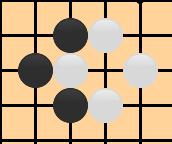
\includegraphics{imgs/ko_rule1.png}
        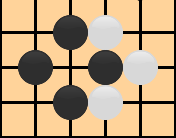
\includegraphics{imgs/ko_rule2.png}
        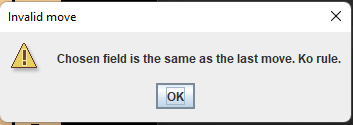
\includegraphics{imgs/ko_rule_warning.png}
    \end{center}
    \item Zasada Superko
    W grze nie może 
    \item Samobójstwo
    Zakładam, że nie jest możliwe popełnienie samobójstwa tj. nie można
    ruszyć się na miejsce, które doprowadzi do przejęcia kamienia 
    przez przeciwnika. Przy próbie popełnienia samobójstwa użytkownikowi 
    ukaże się okienko informujące o zaistniałej sytuacji.

    \item Koniec gry
    Gra kończy się w momencie, w którym nie ma już żadnych ruchów, które 
    nie zakończyłyby się samobójstwem, lub jeden z graczy zrezygnuje z gry, 
    albo oboje graczy przekażą swój ruch pod rząd.

    \item "Martwe" kamienie
    Niemożliwa, jest implementacja algorytmu definiująca 
    "martwe kamienie", dlatego po zakończeniu gry użytkownikowi
     ukaże się okienko, które umożliwia
    wprowadzenie "martwych" kamieni. "Martwe" kamienie zdefiniowane 
    są jako te, które w późniejszej części gry zostałyby przechwycone przez
    przeciwnika.
    Przykład "martwych" kamieni.
    
    \item Liczenie punktów
    Punkty są liczone, jako miejsca na planszy otoczone wyłącznie
    przez dany kamień. Do oznaczenia punktów także użyłam algorytmu flood fill 
    opartym na BFS.

    \item Zapisywanie stanu gry do plików
    Przy próbie zamknięcia okna, użytkownik zobaczy okienko potwierdzenia
    wyjścia z aplikacji. Stan gry będzie automatycznie zapisywany do plików
    txt.

    \item Diagram klas UML
    
    \item Źródła
    https://en.wikipedia.org/wiki/Rules\_of\_Go
\end{enumerate}
% https://www.youtube.com/watch?v=QYNRvMolN20&t=247s
% https://pixabay.com/pl/vectors/czerwony-przycisk-odznaka-okr%c4%85g-47690/


\end{document}
